\coversection{Berechenbarkeit/predic.png}{Berechenbarkeit}{Predictability is like knowing the path a river takes. The river starts at its source and flows down to the sea. Along the way, it may turn, twist, and divide, but it always follows the path of least resistance due to gravity. Knowing the terrain allows us to predict where the river will go.\\ \hspace*{\fill} - ChatGPT}

\textbf{Konvention: } Sprechen wir von einer $e \in \mathbb{N}_0$ oder $(e_1, \cdots, e_n) \in \mathbb{N}_0^n$ wobei $n \in \mathbb{N}$ als Eingabe für eine TM oder Ausgabe einer TM, so bedetet dies, dass die Eingabe bzw. Ausgabe $bin(e)$ bzw $(bin(e_1), \cdots, bin(e_n))$ ist. Dies erlaubt es über partiell berechnenbare Funktionene $\Phi: \mathbb{N}_0^n \leadsto \mathbb{N}_0$ wobei $n\in \mathbb{N}$ zu sprechen und $L \subseteq \mathbb{N}_0$ als Sprache über $\{0, 1\}$ aufzufassen.

\mysubsection{Definition (Code)} Wir betrachten die Funktion code (mit geeignetem Definitionsbereich) und Zielmenge $\{0, 1\}^*$, für die folgendes gilt. Zunächst gelte \[code(L) = 10 \qquad code (S) = 00 \qquad code(R) = 01\] Für eine Instruktion $ I = (q, a, q', a', B) \in \mathbb{N}_0 \times \{0, 1\} \to \mathbb{N}_0 \times \{0, 1\} \times \{L, S, R\}$ einer normierten TM sei \[code (I) = 0^{|bin(q)|} 1 bin (q) a 0^{|bin(q')|} 1 bin (q') a' code (B)\] Für eine endliche Menge $ \Delta \subseteq \mathbb{N}_0 \times \{0, 1\} \to \mathbb{N}_0 \times \{0, 1\}\times \{L, S, R\}$ von Instruktionen einer normierten TM und $i \in [|\Delta|]$ sein $code_i(\Delta)$ dann ein längenlexikographische Ordnung i-te Wort in $\{code(I): I \in \Delta\}$ und sei \[ code (\Delta) = code_1(\Delta), \cdots, code_{|\Delta|}(\Delta)\] Für eine normierte TM $M = (\{0, \cdots, n\}, \{0, 1\}, \{\Box, 0, 1\}, \Delta, 0, \{0\})$ sei \[ code (M) = 0^{|bin(n)|} 1 bin (n) code (\Delta)\] der \textbf{Code} von $M$. Relevant ist hierbei dass es eine geeignete effektive Codierung von Turingmachinen durch Binärwörter gibt, so dass folgendes gilt 
\begin{itemize}
  \item Jede normierte TM hat einen Code 
  \item Keine zwei verschiedene normierten TMs haben den gleichen Code.
  \item Die Sprache der Codes von Turingmachinen ist entscheidbar
  \item Codes können eine geeignete Repräsentation der durch sie codierten TMs umgewandelt werden, die es insbesondere erlauben die codierten TMs effekiv zu simulieren.
  \item geignete Repräsentationen von TMs können effektiv in ihre Codes umgewandet werden.
\end{itemize}

\mysubsection{Definition (standardaufzählung)} Sei $\hat{w_0}, \hat{w_1}, \cdots$ die Aufzählung aller Codes normierter TMs in längenlexikographischer Ordnung. Für $e \in \mathbb{N}_0$ sei $M_e$ die durch $\hat{w_e}$ codierte TM und für $n \in \mathbb{N}$ sei $\Phi_e^n : \mathbb{N}_0^n \rightarrow \mathbb{N}_0$ die von $M_e$ berechnete n-äre partielle Funktion. Für $n \in \mathbb{N}$ heißt die Folge $(\Phi_e^n)$ mit $e\in \mathbb{N}$ \textbf{standardaufzählung} der n-ären partiell berechenbaren Funktion. Für $n \in \mathbb{N} $ und eine partiell berechenbare n-äre Funktion $\varphi: \mathbb{N}_0^n \rightarrow \mathbb{N}_0$ heißt jede zahl $e \in \mathbb{N}_0$ mit $\Phi_e^n = \varphi$ \textbf{Index} von $\varphi$.

\textbf{Konvention: } Ergibt sich n aus dem Kontext, so schreiben wir auch $\Phi_e$ statt $\Phi_e^n$

\mysubsection{Bemerkung} Für $n \in \mathbb{N}$ und eine partielle berechnbare n-äre partielle Funktion $\Phi : \mathbb{N}_0^n \rightarrow \mathbb{N}_0$ gibt es unendlich viele Indizes von $\varphi$.

\mysubsection{Definition (U)} Es bezeichnet U die normierte TM, die bei Eingabe $(e, x_1, \cdots, x_n) \in \mathbb{N}_0^{n+1}$ wobei $n \in \mathbb{N}$ die normierte TM $\mathcal{M}_e$ bei Eingabe $(x_1, \cdots, x_n)$ simuliert und falls diese terminiert die Ausgabe der Simulierten ausgibt.

\mysubsection{Definition (Universell)} Eine DTM U heißt \textbf{Universell}, wenn es für alle $n \in \mathbb{N}$ und alle partiell berechenbaren Funktionen $\varphi : \mathbb{N}_0^n \leadsto \mathbb{N}_0$ eine $e \in \mathbb{N}$, so dass \[U(e, x_1, \cdots, x_n) = \varphi(x_1, \cdots, x_n)\] $\forall x_1, \cdots, x_n \in \mathbb{N}_0$ gilt.

\mysubsection{Bemerkung} \sloppy Die TM U ist universell, denn für $e \in \mathbb{N}_0$, $n \in \mathbb{N}$ und $x_1, \cdots, x_n \in \mathbb{N}_0$ gilt \[U(e,x_1, \cdots, x_n) = \Phi_e(x_1, \cdots, x_n)\]\\ \[(x, y) \mapsto x^y\] \[y \mapsto 2^y\] \[(x_1, \cdots, x_m, y_1, \cdots, y_n) \mapsto \varphi(x_1, \cdots, x_m, y_1, \cdots, y_n) partiell berechenbar\] \[\leadsto (y_1,\cdots, y_m) \mapsto \varphi(x_1, \cdots, x_m, y_1, \cdots, y_n) partiell berechenbar \]

\mysubsection{Satz ($s_n^m$ - Theorem)} 
$\forall m, n \in \mathbb{N}$ existiert eine berechenbare Funktion $s_n^m : \mathbb{N}_0^{m+1} \to \mathbb{N}_0$  mit \[\Phi_e^{m+1}(x_1\cdots, x_m, y_1, \cdots, y_n) = \Phi_{s_n^m(e, x_1, \cdots, x_m)}^n (y_1, \cdots, y_n)\] $\forall e, x_1, \cdots, x_m, y_1, \cdots, y_n \in \mathbb{N}_0$

\begin{proof}Fixiere $m \in \mathbb{N}$. Betrachte die DTM S , die bei Eingabe $(e, x_1, \cdots, x_m) \in \mathbb{N}_0^{m+1}$ wie folgt vorfährt.
\begin{itemize}
  \item Zunächst bestimmt S den Code von $\mathcal{M}_e$ 
  \item der Code von $\mathcal{M_e}$wird dann in einen Code einer normierten TM $\mathcal{M}$ umgewandet, die zunächst $x_1\Box\cdots\Box x_m\Box$ neben die Eingabe schreibt, dan den Kopf auf das erste Feld des beschriebenen Bandteilsbewegt und dann wie $\mathcal{M_e}$ arbeitet.
  \item Es wird bestimmt an welcher Stelle der Standardaufzählung der Code von auftaucht und diese Stelle wird ausgegeben.
\end{itemize}
Sei $s_n^m$ die von S berechnete $(m+1)$-äre partielle Funktion. Dann ist $s_n^m$ eine Funktion wie gewünscht. Es gibt überabzählbar viele Binärsprachen, denn: Betrachte Aufzählung von Binärsprachen $L_1, L_2, \cdots$ 
\begin{table}[ht]
  \centering
  \renewcommand{\arraystretch}{2} % Adjust the value to increase or decrease the cell size
  \begin{tabular}{c c c c c}
    \tikzmarknode{L0-0}{$\mathds{1}_{L_0}(0)$} & $\mathds{1}_{L_0}(1)$ & $\mathds{1}_{L_0}(2)$ & $\mathds{1}_{L_0}(3)$ \\
    $\mathds{1}_{L_1}(0)$ & $\mathds{1}_{L_1}(1)$ & $\mathds{1}_{L_1}(2)$ & $\mathds{1}_{L_1}(3)$ \\
    $\mathds{1}_{L_2}(0)$ & $\mathds{1}_{L_2}(1)$ & \tikzmarknode{L2-2}{$\mathds{1}_{L_2}(2)$} & $\mathds{1}_{L_2}(3)$ \\
  \end{tabular}
  \captionsetup{labelformat=empty, justification=centering, skip=10pt}
  \caption{Standardaufzählung}
  
  \begin{tikzpicture}[overlay, remember picture, red, >=stealth]
    \draw [->, thick] ([yshift=1ex]L0-0.south) -- ([yshift=-1ex]L2-2.north);
  \end{tikzpicture}
\end{table}

$L$ mit $\mathds{1}_L(i)$ = 
$\begin{cases}
    0, & \text{wenn } \mathds{1}_{L_i}(i) = 1 \\
    1, & \text{wenn } \mathds{1}_{L_i}(i) = 0 \\
\end{cases}$
\end{proof}

\mysubsection{Definition (diagonales Halteproblem)} Die Menge $H_{diag} := \{e \in \mathbb{N}_0 : \Phi_e (e) \downarrow\}$ heißt \textbf{diagonales Halteproblem}.

\mysubsection{Proposition} Das diagonale Halteproblem ist rekursiv aufzählbar.
\begin{proof}
  Die DTM, die bei Eingabe $e \in \mathbb{N}_0$ wie $U$ bei Eingabe $(e, e)$ arbeitet, aber bei terminieren $1$ statt der Ausgabe von $U$ ausgibt berechnet die partielle charachteristische Funktion von $H_{diag}$. Die partielle Funktion $x_{H_{diag}}$ ist also partiell berechenbar. Die partielle Funktion $x_{H_{diag}^c}$ ist nicht partiell berechenbar, dann: Betrachte Standardaufzählung
\end {proof}
  
\begin{table}[ht]
  \centering
  \renewcommand{\arraystretch}{2} % Adjust the value to increase or decrease the cell size
  \begin{tabular}{c c c c c}
    \tikzmarknode{L0-0}{$\Phi_{L_0}(0)$} & $\Phi_{L_0}(1)$ & $\Phi_{L_0}(2)$ & $\Phi_{L_0}(3)$ \\
    $\Phi_{L_1}(0)$ & $\Phi_{L_1}(1)$ & $\Phi_{L_1}(2)$ & $\Phi_{L_1}(3)$ \\
    $\Phi_{L_2}(0)$ & $\Phi_{L_2}(1)$ & \tikzmarknode{L2-2}{$\Phi_{L_2}(2)$} & $\Phi_{L_2}(3)$ \\
  \end{tabular}
  \captionsetup{labelformat=empty, justification=centering, skip=10pt}
  \caption{Standardaufzählung}
\end{table}

\begin{tikzpicture}[overlay, remember picture, green, >=stealth]
  \draw [->, thick] ([yshift=1ex]L0-0.south) -- ([yshift=-1ex]L2-2.north);
\end{tikzpicture}

$\varphi$ mit $\varphi(i)$ = 
$\begin{cases}
    \uparrow, & \text{wenn } \Phi_i(i) \downarrow\\
    \downarrow, & \text{wenn } \Phi_i(i) \uparrow \\
\end{cases}$
Wird nicht aufgezählt.

\mysubsection{Satz} Das diagonale Halteproblem ist nicht entscheidbar. 
\begin{proof}
  Angenommen $H_{diag}$ wäre entscheidbar. Dann wäre die partielle charakteristische Funktion $\varphi$ von $H_{diag}^c = \mathbb{N}_0 / H_{diag}$ partiell berechenbar, es gäbe also ein Index $e \in \mathbb{N}_0$ von $\varphi$. Es folge \[e \in H_{diag}^c \Leftrightarrow \varphi(e) \downarrow \Leftrightarrow \Phi_e(e) \downarrow \Leftrightarrow e \in H_{diag} \Leftrightarrow e \not \in H_{diag}^c\] Die ist ein Wiederspruch.
\end{proof}

\mysubsection{m-Reduktion} Für eine Sprache $A$ über einem Alphabet $\Sigma$ und eine Sprache $B$ über einem Alphabet $\Gamma$ ist A genau dann \textbf{many-one-reduzierbar}, auch \textbf{m-reduzierbar}, auf $B$, kurz $A \leq_m B$, wenn es eine berechebare Funktion. $f: \Sigma^* \to \Gamma^*$ gibt so dass \[w \in A \Leftrightarrow f(w)\in B\] $\forall w \in \Sigma^*$ gilt. Gelten $A \leq_m B$ und $B \leq_{m} A$, so sind $A$ und $B$ \textbf{many-one-äquivalent} auch \textbf{m-äquivalent}, kurz $A =_m B$.

\mysubsection{Bemerkung} 
\begin{itemize}
  \item [(i)] $\leq_m$ ist transitiv.
  \item [(ii)] Gilt $A \leq_m B$ für Sprachen $A$ und $B$ und ist $B$ entscheidbar, so ist auch $A$ entscheidbar.
  \item [(iii)] Alle entscheidbaren Sprachen L mit $\varnothing \not = L \not = \mathbb{N}_0$ und m-äquivalent.
\end{itemize}

\mysubsection{Satz} Das \textbf{initiale Halteproblem} $H_{init} = {e \in \mathbb{N}_0 = \Phi_e(0) \downarrow}$ ist nicht entscheidbar.

\subsubsection*{Idee: } suche $f:\mathbb{N}_0 \to \mathbb{N}_0$ mit $\Phi_e(e)\downarrow \Leftrightarrow \Phi_{f(e)}(0)\downarrow$ Wähle $f$ so dass $\Phi_{f(e)}(x) = \Phi_e(e)$ $\forall x \in \mathbb{N}_0$

\begin{proof}
  Sei $\psi : \mathbb{N}_0^2 \leadsto \mathbb{N}_0$ mit $\psi (e, x) = \Phi_e(e) \forall e, x \in \mathbb{N}_0$. Dann ist $\psi$ partiell berechenbar. Sei $e_0$ ein Index von $\psi$ und $s:\mathbb{N}_0^2 \to \mathbb{N}_0$ gilt. Sei $f: \mathbb{N}_0 \to \mathbb{N}_0$ mit $f(e) = s(e_0, e) \forall e /in \mathbb{N}_0$. Dann ist f berechenbar. $\forall e \in \mathbb{N}_0$ gilt. \[e \in H_{diag} \Leftrightarrow \Phi_e(e) \downarrow \Leftrightarrow \psi(e, 0) \downarrow \Leftrightarrow \Phi_{e_0}(e, 0) \downarrow \Leftrightarrow \Phi_s (e_0, e)(0)\downarrow \Leftrightarrow \Phi_{f(e)} (0)\downarrow \Leftrightarrow f(e) \in H_{init}\] Es gilt also $H_{diag} \leq_{m} H_{init}$, da $H_{diag}$ nicht entscheidbar ist, ist damit $H_{init}$ nicht entscheidbar.
\end{proof}

\textbf{Dominosteinspiel!}
\subsubsection*{Gegeben: } Endlich viele typen von Spielsteinen mit jeweils zwei beschrifteten Feldern: "oberes Feld, unteres Feld". Beschritungen sind nichtleere Wörter über einem Alphabet. Spielsteine sind vom gleichen Typ, wenn die beiden oberen Felder gleich beschriftet sind und die beiden unteren Felder gleich beschriftet sind. Es gibt von jedem Typ beliebig viele steine. 

\subsubsection*{Gesucht: }Können ein oder mehrere (aber endlich viele) Spielsteine so nebeneinander gelegt werden, dass sich oben und unten von links nach rechts gelesen das gleiche Wort ergibt?
\begin{center}
  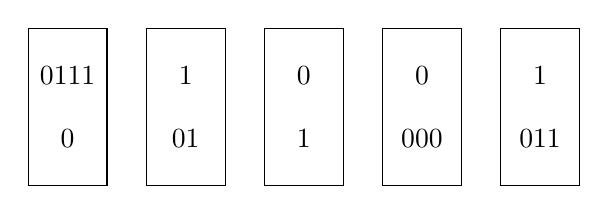
\begin{tikzpicture}
    % Define styles for Dominoes
    \tikzstyle{domino}=[rectangle, draw, minimum width=1cm, minimum height=2cm, inner sep=0pt]
  
    % Domino (0111, 0)
    \node[domino] (d1) at (0,0) {};
    \node at ([yshift=4mm]d1.center) {0111};
    \node at ([yshift=-4mm]d1.center) {0};
  
    % Domino (1, 01)
    \node[domino] (d2) at (1.5,0) {};
    \node at ([yshift=4mm]d2.center) {1};
    \node at ([yshift=-4mm]d2.center) {01};
  
    % Domino (0, 1)
    \node[domino] (d3) at (3,0) {};
    \node at ([yshift=4mm]d3.center) {0};
    \node at ([yshift=-4mm]d3.center) {1};
  
    % Domino (0, 000)
    \node[domino] (d4) at (4.5,0) {};
    \node at ([yshift=4mm]d4.center) {0};
    \node at ([yshift=-4mm]d4.center) {000};
  
    % Domino (1, 011)
    \node[domino] (d5) at (6,0) {};
    \node at ([yshift=4mm]d5.center) {1};
    \node at ([yshift=-4mm]d5.center) {011};
  
    \end{tikzpicture}
    \vspace{1cm}\\
    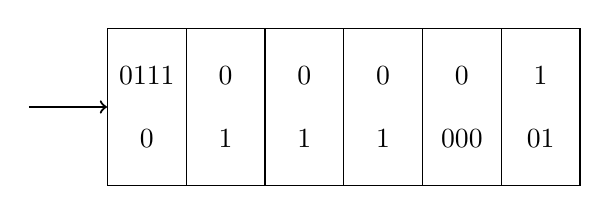
\begin{tikzpicture}

      % Define styles for Dominoes
      \tikzstyle{domino}=[rectangle, draw, minimum width=1cm, minimum height=2cm, inner sep=0pt]
      
      % Domino (0111, 0)
      \node[domino] (d1) at (0,0) {};
      \node at ([yshift=4mm]d1.center) {0111};
      \node at ([yshift=-4mm]d1.center) {0};
      
      % Domino (0, 1)
      \node[domino] (d2) at (1,0) {};
      \node at ([yshift=4mm]d2.center) {0};
      \node at ([yshift=-4mm]d2.center) {1};
      
      % Domino (0, 1)
      \node[domino] (d3) at (2,0) {};
      \node at ([yshift=4mm]d3.center) {0};
      \node at ([yshift=-4mm]d3.center) {1};
      
      % Domino (0, 1)
      \node[domino] (d4) at (3,0) {};
      \node at ([yshift=4mm]d4.center) {0};
      \node at ([yshift=-4mm]d4.center) {1};
      
      % Domino (0, 000)
      \node[domino] (d5) at (4,0) {};
      \node at ([yshift=4mm]d5.center) {0};
      \node at ([yshift=-4mm]d5.center) {000};
      
      % Domino (1, 01)
      \node[domino] (d6) at (5,0) {};
      \node at ([yshift=4mm]d6.center) {1};
      \node at ([yshift=-4mm]d6.center) {01};
      
      % Arrow pointing to the leftmost domino
      \draw[->, thick] (-1.5,0) -- (d1.west);

      \end{tikzpicture}
        
  \end{center}

  \mysubsection{Definition (Postsches Korrespondenzproblem, Emil Port, 1946)} Für ein Alphabet $\Sigma$ sei eine Instanz des Postschen Korrespondenzproblems über $\Sigma$ eine endliche Teilmenge $I \subseteq (\Sigma^+)^2$. Eine Lösung für eine solche Instanz ist eine endliche Folge $(u_1, v_1), \cdots, (u_n, v_n)$ von Paaren in $I$ mit $n \geq 1$,so dass \[u_1 \cdots u_n = v_1 \cdots v_n\] Gibt es eine Lösung für eine instanz des Postschen Korrespondenzproblems, so heißt diese Instanz lösbar. Das \textbf{Postsche Korrespondenzproblem} über einem Alphabet $\Sigma$, kurz $PCP_{\Sigma}$ ist die Menge aller lösbaren Instanzen des Postschen Korrespondenzproblems über $\Sigma$.\\\\ Für ein Alphabet $\Sigma$ sei eine Instanz des modifizierten Postschen Korrespondenzproblems über $\Sigma$ ein Paar $(p, I)$, wobei $I\subseteq (\Sigma^+)^2$ eine endliche Teilmenge und $p\in I$ ein Paar von Wörtern ist. Eine Lösung für eine solche Instanz ist eine endlcihe Folge $(u_1, v_1), \cdots, (u_n, v_n)$ von Paaren ist $I$, so dass \[p = (u_1, v_1) und u_1\cdots u_n = v_1\cdots v_n\] Gibt es eine Lösung für eine Instanz des modifizierten Postschen Korrespondenzproblems so heißt diese Instanz lösbar. Das \textbf{modifizierte Postsche Korrespondenzproblem} über einem Alphabet $\Sigma$, kurz $MPCP_{\Sigma}$ ist die Menge aller lösbaren Instanzen des modifizierten Postschen Korrespondenzproblems über $\Sigma$.
  \subsubsection*{Plan: } Für Alphabet mit $|\Sigma| \geq 2$: \[H_{init} \stackrel{(3)}{\leq_m} MPCP_{\Gamma} \stackrel{(2)}{\leq_m} PCP_{\Gamma} \stackrel{(1)}{\leq_m} PCP_{\Sigma}\]
  \mysubsection{Lemma} Für ein Alphabet $\Sigma$ und $\Gamma$ mit $|\Sigma| \geq w$ gilt $PCP_{\Gamma} \leq_m PCP_{\Sigma}$
  \begin{proof}
    Wir suchen eine effektive Transformation, die jede Instanz $I$ des Postschen Korrespondenzproblems über $\Gamma$ in eine Instanz $I'$ des postschen Korrespondenzproblems über $\Sigma$ transformiert, so dass $I$ genau dann lösbar ist, wenn $I'$ lösbar ist. Seien $a_1, a_2 \in \Sigma$ verschieden und sein $b_1, \cdots, b_{|\Gamma|}$ die Elemente von $\Gamma$. Es bezeichne $\varphi : \Gamma^* \to \Gamma^*$ den eindeutigen Homomorphismus von Sprachen mit $\varphi (b_i) = a^i_1 a_2$ $\forall i \in [|\Gamma|]$. Gegeben eine solche Instanz $I$ wie oben sei $I' := \{(\varphi(u), \varphi(v)) : (u, v) \in I\}$. Die Funktion, die geeignete Codes von Instanzen $I$ auf geeignete Codes von Instanzen $I'$ abbildet ist berechenbar. Ist $(u_1, v_1), \cdots, (u_n, v_n)$ eine lösung $I$, so gilt \[\varphi(u_1) \cdots \varphi(v_1) = \varphi(u_1, \cdots, \varphi(v_n)) = \varphi(v_1, \cdots, v_n) = \varphi(v_1) \cdots \varphi(v_n)\] und somit ist $(\varphi(u_1), \varphi(v_1), \cdots, (\varphi(u_n)), \varphi(v_n))$ eine Lösung von $I'$. Die Instanz $I'$ ist also lösbar wenn $I$ lösbar ist. Ist $(u'_1, v'_1), \cdots, (u'_n, v'_n)$ eine Lösung von $I'$, so gibt es eine Folge $(u_1, v_1)\cdots (u_n, v_n)$ von Paaren in $I$ mit $\varphi(u'_i)$ und $\varphi(v_i) = v'_i$ $\forall i \in [n]$, also mit \[\varphi(u_1, \cdots, u_n) = u'_1, \cdots, u'_n = u'_1, \cdots, u'_n =\varphi(u_1, \cdots, u_n)\] Da $\varphi \vert_{\Sigma}$ injektiv und $\varphi (\Sigma)$ präfixfrei ist, ist $\varphi$ injektiv (siehe Übung), folglich gilt $u_1, \cdots, u_n = v_1, \cdots, v_n$ und somit ist $(u_1, v_1), \cdots, (u_n, v_n)$ eine Lösung von $I$. Die Instanz $I$ ist also lösbar wenn $I'$ Lösbar ist.
  \end{proof}


  \mysubsection{Lemma} Für Jedes alphabet $\Sigma$ mit $|\Sigma| \leq w$ gitl $MPCP_{\Sigma} \leq_m PCP_{\Sigma}$.
  \begin{proof}
    Sei $\Sigma$ ein Alphabet mit $|\Sigma| \geq 2$. Nach \hyperref[subsec:3.14]{Lemma 3.14}  genügt es ein Alphabet $\Gamma$ zu finden, so das $MPCP_{\Sigma} \leq_m PCP_{\Gamma}$ gilt. \\Wir suchen eine effektive Transformation , die jede instanz $(p, I)$ des modifizierten Postschen Korrespondenzproblems über $\Sigma$ in eine Instanz $I'$ des Postschen Korrespondenzproblems über einem geeignetem Alphabet$\Gamma$ transformiert, so dass $(p, I)$ genau dann lösbar ist, wenn $I'$ lösbar ist.
  \end{proof}
  \subsubsection*{Idee: }
  \begin{center}
    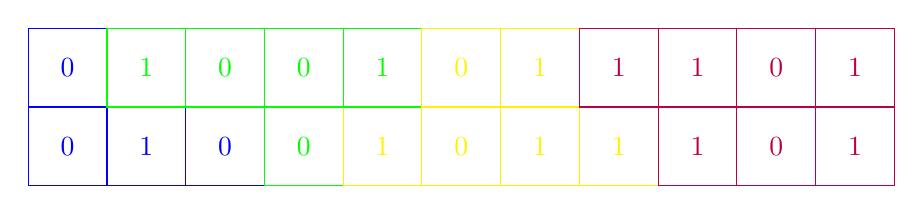
\begin{tikzpicture}
      \draw[blue] (0,0) rectangle (1,1) node[midway] {0};
      \draw[blue] (1,0) rectangle (2,1) node[midway] {1};
      \draw[blue] (2,0) rectangle (3,1) node[midway] {0};
      \draw[green] (3,0) rectangle (4,1) node[midway] {0};
      \draw[yellow] (4,0) rectangle (5,1) node[midway] {1};
      \draw[yellow] (5,0) rectangle (6,1) node[midway] {0};
      \draw[yellow] (6,0) rectangle (7,1) node[midway] {1};
      \draw[yellow] (7,0) rectangle (8,1) node[midway] {1};
      \draw[purple] (8,0) rectangle (9,1) node[midway] {1};
      \draw[purple] (9,0) rectangle (10,1) node[midway] {0};
      \draw[purple] (10,0) rectangle (11,1) node[midway] {1};
  
      \draw[blue] (0,1) rectangle (1,2) node[midway] {0};
      \draw[green] (1,1) rectangle (2,2) node[midway] {1};
      \draw[green] (2,1) rectangle (3,2) node[midway] {0};
      \draw[green] (3,1) rectangle (4,2) node[midway] {0};
      \draw[green] (4,1) rectangle (5,2) node[midway] {1};
      \draw[yellow] (5,1) rectangle (6,2) node[midway] {0};
      \draw[yellow] (6,1) rectangle (7,2) node[midway] {1};
      \draw[purple] (7,1) rectangle (8,2) node[midway] {1};
      \draw[purple] (8,1) rectangle (9,2) node[midway] {1};
      \draw[purple] (9,1) rectangle (10,2) node[midway] {0};
      \draw[purple] (10,1) rectangle (11,2) node[midway] {1};
    \end{tikzpicture}
  \end{center}
  ...
  Betrachte die Homomorphismus von Sprachen $\delta_{\rightarrow}$, $\delta_{\leftarrow} : \Sigma^* \rightarrow (\Sigma \cup {*})^*$ mit $\delta_{a} = a*$ und $\delta_{\leftarrow}(a) = *a$ $\forall a \in \Sigma$. Für jede Instanz $(p, I) = ((u_1, v_1), I)$ wie oben sei \[I' = \{(\delta_{\leftarrow}(u_1), *\delta_{\rightarrow}(v_1))\} \cup \{\delta_{leftarrow}(u), \delta_{rightarrow}(v):  (u, v) \in I\} \cup \{\delta_{\leftarrow}(u)*, \delta_{\rightarrow}(v): (u, v) \in I\}\] Die Funktion die geeignete Codes von Instanzen $(p, I)$ auf geeignete Codes der zugehörigen Instanzen $I'$ abbildet ist berechenbar. Gibt es eine Lösung $(u_1, v_1), \cdots, (u_n, u_n)$ von $(p,I)$ dann ist \[\delta_{\leftarrow}(u_1)\cdots \delta_{\leftarrow}(u_n)* = \delta_{\leftarrow} (u_1 \cdots u_n)*\]
  \[= \delta_{\leftarrow}(v_1 \cdots v_n)*\] \[= *\delta_{\rightarrow}(v_1 \cdots v_n)\] \[=*\delta_{\rightarrow}(v_1) \cdots \delta_{\rightarrow}(v_n)\] und folglich ist \[(\delta_{\leftarrow}(u_1), *\delta_{\rightarrow}(v_1)), (\delta_{\leftarrow}(u_2), \delta_{\rightarrow}(v_2)), \cdots, (\delta_{\leftarrow}(u_{n-1}), \delta_{\rightarrow}(v_{n-1})), (\delta_{\leftarrow}(u_{n}), \delta_{\rightarrow}(v_{n}))\] eine Lösung von $I'$. Es bleibt zu zeigen das $(p, I)$ lösbar ist, wenn $I'$ lösbar ist. Sei $\tau : (\Sigma \cup \{*\})^* \rightarrow \Sigma^*$ der Homomorphismus von Sprachen mit $\tau \vert_{\Sigma} = id_{\Sigma}$ und $\tau(*) = \lambda$. Für $(u', v') \in I'$ gilt $(\tau (u'), \tau(v')) \in I$. Sei $(u'_1, v'_1), \cdots, (u'_n, v'_n)$ eine Lösung von $I'$ und $(u'_i, v'_i) = (\tau(u'_i), \tau(v'_i))$ für $i \in [n]$. Es gilt \[\tau(u'_1) \cdots \tau(u'_n) = \tau(u'_1 \cdots u'_n) = \tau(v'_1 \cdots v'_n) = \tau(v'_1) \cdots \tau(v'_n)\] und somit ist $(u_1, v_1), \cdots, (u_n, u_v)$ eine Lösung von $I$ als Instanz des Postschen Korrespondenzproblems über $\Sigma$. Es genügt aber zu zeigen, dass $(u_1, v_1) = p $ gilt. Sei $p' = (\delta_{\leftarrow} (u_1), \not \tau (?wirklich nicht tau?) \delta_{\rightarrow}(v_1))$. Für $(u', v') \in I' / \{p'\}$ gilt $u'(1) \not = v'(1)$, da $(u'_1, v'_1), \cdots, (u'_n, v'_n)$ eine Lösung von $I'$ ist gilt also $(u'_1, v'_1) = p'$ und damit $(u_1, v_1) = (\tau(u'_1), \tau(v'_1)) = p$.

  \mysubsection{Lemma}
  Für jedes Alphabet $\Sigma$ mit $|\Sigma| \geq 2$ gilt $H_{init} \leq_m MPCP_{\Box, 0, 1, *, 6, +}$

  \begin{proof}
    Wir suchen eine effektive Transformation, die jede natürliche Zahl $e$ auf eine Instanz $(p_e,I_e)$ des modifizierten Portschen Korrespondenzproblems über $\{\Box, 0, 1, *, , +\}$ abbildet, so dass $\mathcal{M} _e(\lambda)\downarrow$ genau dann gilt, wenn $(p_e, I_e)$ lösbar ist. Sei $e \in \mathbb{N}_0$. Sei $Q$ Die Zustandsmenge und $\Delta$ die Übergangsrelation von $\mathcal{M}_e$. Es gelte also $\mathcal{M}_e = (Q, \Sigma, \Gamma, \Delta, s, F)$ für $\Sigma = \{0, 1\}$, $\Gamma = \{\Box, 0, 1\}$, $S = 0$, $F = \{0\}$ \\ Für eine Instanz $(p, I)$ des modifizierten Postschen Korrespondenzproblems über einem Alphabet bezeichnen wir eine Folge $p =  (u_1, v_1), \cdots, (u_n, v_n)$ für die $u_1 \cdots u_n \sqsubseteq v_1 \cdots v_n$ oder $v_1 \cdots v_n \sqsubset u_1 \cdots u_n$ gilt als \textbf{partielle Lösung} von $(p, I)$. Wir wollen $(p_e, I_e)$ so wählen, dass partielle Lösungen von $(p_e, I_e)$ partielle Rechungen von $\mathcal{M}_e$ entsprechen. Dabei codieren wie eine Konfiguration $(p, w, p) \in Q \times(\Gamma^*)*\mathbb{N}_0$ von $\mathcal{M}_e$ durch das Wort \[code (q, w, p) := \# w(1)\cdots w(p-q) * bin(q)* w(p) \cdots w(|w|)\#\] Im wesentlichen wollen wir erreichen, dass es genau dann für ein Wort w eine partielle lösung  $(u_1, v_1), \cdots, (u_n, v_n)$ von $(p_e, I_e)$ mit $w = v_1 \cdots v_n$ gibt, wenn $w$ Präfix der Konkation $code (C_1) \cdots code (C_n)$ der Code der Konfiguration einer partiellen Rechnung $C_1, \cdots, C_n$ von $\mathcal{M}_e$ bei Eingabe $\lambda$ ist. Eine solche partielle Lösung soll genau dann zu einer Lösung von $(p_e, I_e)$ vervollständigt werden können, wenn die durch $w$ beschriebene partielle Rechung mit einer Stoppkonfiguraion endet, alsp eine Rechung ist. Dann ist $(p_e, I_e)$ genau dann lösbar, wenn die Rechung von $\mathcal{M}_e$ zur Eingabe $\lambda$ endlich ist. \\\\ Für $q \in Q$ sei $\hat{q} : * bin(q)$\\ Als Startpaar sehen wir \[p_e = (0, 0 \# * \ *\Box\#)\] (die 0en sind nur dafür da da, damit "im?" komplment nicht leer ist.) Wir beschreiben nun die Konstruktion von $I_e$. Für jede Instruktion $(q, a, q', a', L) \in \Delta$ fügen wir folgende Paare ein \[(\# \hat{q}a, \# \hat{q}'\Box a'), (\Box \hat{q} a, \hat{q}'\Box a'), (0\hat{q}a, \hat{q}'0a')(1\hat{q}a, \hat{q}'1a')\] ein. Weiter, um unveränderte Infixe kopieren zu können fügen wir die Paare \[(\#, \#), (0, 0), (1,1), (\Box, \Box)\] ein. Nun brauchen wir noch Paare, die bei Terminierung der TM zu einer validen Instanz der $MPCP$ - Instanz führen.\\ $\leadsto \forall q \in Q \forall a \in \{\Box, 0, 1\}$ für die es keine Instruktion $(q, a, q', a', B)$ fürgen wir das Paar $(\hat{q}a, \dagger a)$ hinzu und auch \[(\dagger \Box, \dagger), (\dagger 0, \dagger), (\dagger 1, \dagger)\] \[(\Box \dagger, \dagger),(0 \dagger, \dagger),(1\dagger, \dagger)\] \[(\# \dagger \# 0, 0)\] Dies beschreibt die Konstruktion von $(p_e, I_e)$. Wir verzichten auf die einfache aber aufwändige Verfifikation, dass $\mathcal{M}_e$ genau dann bei Eingabe $\lambda$ terminiert, wenn $(p_e, I_e)$ lösbar ist.
  \end{proof}
  \mysubsection{Beispiel} Sei $e \in \mathbb{N}_0$ mit $\mathcal{M}_e = (\{0, 1\}, \{0, 1\}, \{\Box, 0, 1\}, \Delta, 0, \{0\})$, wobei $\Delta = \{(0, \Box, 1, 1, R), (1, \Box, 1, 1, L)\}$. Mitder Notation aus dem Beweis aus \hyperref[subsec:3.16]{Lemma 3.17} gilt dann [hier bild einfügen!]

  \mysubsection{Satz} Für jedes Alphabet $\Sigma$ mit $|\Sigma| \geq 2$ ist $PCP_{\Sigma}$ nicht entscheidbar. 
  \begin{proof}
    Mit \hyperref[subsec:3.16]{Lemma 3.16}, \hyperref[subsec:3.17]{Lemma 3.17} und \hyperref[subsec:3.18]{Lemma 3.18} folgt \[H_{init} \leq_m MPCP_{\Box, 0, 1, *, \#, \dagger} \leq_m PCP_{\Box, 0, 1, *, \#, \dagger} \leq_m PCP_{\Sigma}\] und damit $H_{init} \leq_m PCP_{\Sigma}$. Folglich ist $PCP_{\Sigma}$ nicht entscheidbar, da $H_{init}$ nicht entscheidbar ist.
  \end{proof}

  %alda
  \mysubsection{Fixpunktsatz, Rekusionstheorem und Satz von Rice} 
  
  Wir beschäftigen uns nun mit weiteren Konsequenzen der Standardaufzählung von TM. \[ \Phi_0, \Phi_1, \Phi_2, \cdots \] Standardaufzählung \[\Phi_{\Phi_e(0)}, \Phi_{\Phi_e(1)}, \Phi_{\Phi_e(2)}, \cdots\] andere Aufzählung $\Rightarrow$ \[\Phi_{f(0)}, \Phi_{f(1)}, \Phi_{f(2)}\]

  \mysubsubsection{Definition (Fixpunktsatz)} Ein \textbf{Fixpunkt} eine berechenbaren Funktion $f: \mathbb{N}_0 \to \mathbb{N}_0$ ist ein $e \in \mathbb{N}_0$ mit $\Phi_{f(e)} = \Phi_e$.

  \mysubsubsection{Satz (Fixpunktsatz, Hartley Rogers jr., 1967)} Alle berechenbaren Funktionen $f : \mathbb{N}_0 \to \mathbb{N}_0$ haben einen Fixpunkt.
  \begin{proof}
    $\forall e, x \in \mathbb{N}_0$ mit $\Phi_e(x) \uparrow$ sei $\Phi_{\Phi_e(x)} : \mathbb{N}_0 \leadsto \mathbb{N}_0$ die aprtiell berechenabre partielle Funktion mit $dom(\Phi_{\Phi_e(x)}) = \varnothing$. Sei $e_{\psi}$ ein Index von $\psi$. Gemäß $S_n^m$-Theorem (\hyperref[subsec:3.16]{Satz 3.7}) existiert eine berechenbare Funktion $s_1^1 : \mathbb{N}_0^2 \to \mathbb{N}_0$ mit $\Phi_{s_1^1(e_{\psi}, e)}(x) = \psi(e, x)$. $\forall e, x \in \mathbb{N}_0$.Sei $\eta : \mathbb{N}_0 \to \mathbb{N}_0$ die berechenbare Funktion mit $\eta (e) := s_1^1(e_{\psi}, e)$. Dann gilt \[\psi_{\eta(e)}(x) = \psi_{s_1^1(e_{\psi}, e)}(x) = \psi(e, x) = \Phi_{\Phi_e(e)}(x) \forall x \in \mathbb{N}_0\] also gilt \[\Phi_{\eta(e)} = \Phi_{\Phi_e (e)} (*)\] Sei $e_{f \circ h}$ ein Index der berechneten Funktion $f \circ h$ und $e_{fix} := \eta(e_{f\circ h})$. \[ \Phi_{f(e_{fix})} = \Phi_{f(\eta(e_{f \circ h}))} = \Phi_{\Phi{e_{f\circ h}} (e_{f\circ h})} \overset{(*)}{=} \Phi_{\eta(e_{f \circ h})} = \Phi_{e_\eta}\] Folglich ist $e_{fix}$ ein Fixpunkt von $f$. 
  \end{proof}
  Solche Fixpnkte wie oben sind "semandische" Fixpunkte und kein "syntaktischen" Fixpunkte. Aus dem Fixpunktsatz kann man leicht das Rekursionstheorem folgen, dsa es anschaulich erlaubt während der Konstruktion einer partiell berechebaren Funktion anzunehmen den Index der fertig definierten Funktion zu kennen. Auf Programmebene bedeutet das, das es möglich ist ein Programm so zu schreiben ,dass der fertige Quellcode im Programm zur Verfügung stelt (ohne diesen irgendwo, zum Beispiel vom Speicher des Quellcodes, einzulesen)

  \mysubsubsection{Satz (Rekursionstheorem, Stephen Cole Kleen, 1938)} 
  Für alle partielle Funktionen $\varphi : \mathbb{N}_0^2 \leadsto \mathbb{N}_0$ gibt es ein $e \in \mathbb{N}_0$ mit $\Phi_e(x) = \varphi(e, x) \quad \forall x \in \mathbb{N}_0$ 

  \begin{proof}
    Sei $e_{\varphi}$ ein index von $\varphi$. Gemäß $s_n^m$ - Theorem gibt es eine berechenbare Funktion $s_1^1 : \mathbb{N}_0^2 \to \mathbb{N}_0$ mit $\Phi_{s^1_1 (e_{\varphi}, e)} (x) = \varphi (e, x) \quad \forall x \in \mathbb{N}_0$
  \end{proof}

  Für Programme bedeutet dies die Existenz von sogenannten \textbf{Quines}. Dies sind Programme, die ihren eigenen Quellcode ausgeben (ohne diesen vom speicher zu lesen). Unsere Resultate zeigen, dass für hinreichend komplexe Programmiersprachen immer Quines existieren. Eine weitere Konsequent aus dem Fixpunktsatz ist die Einsicht, dass jede nicht triviale Programmiereigenschaft unentscheidbar ist.

  \mysubsubsection{Korollar}
  Es gibt ein $e \in \mathbb{N}_0$ mit $\Phi_e(x) = e \quad \forall x \in \mathbb{N}_0$.
  \begin{proof}
    Sei $\psi : \mathbb{N}_0^2 \leadsto \mathbb{N}_0$ die partiell berechebare Funktion mit $\psi(e, x) = e \quad \forall e, x \in \mathbb{N}_0$. Gemäß \hyperref[subsubsec:3.20.2]{Satz 3.20.2} gibt es nun ein $e \in \mathbb{N}_0$ mit $\Phi_e (x) = \psi (e,x) = e \quad \forall x \in \mathbb{N}_0$
  \end{proof}

  \mysubsubsection{Definition (Indexmenge)} 
  Eine Teilmenge $I \subseteq \mathbb{N}_0$ heißt Indexmenge, wenn $e \in I \Leftrightarrow e' \in I \quad \forall e, e' \in \mathbb{N}_0$ mit $\Phi_e = \Phi_e'$ gilt.

  \mysubsubsection{Satz (Satz von Rice, Henry Horden Rice, 1951)}
  Ist $I$ ein Indexmenge $\varnothing \not = I \not = \mathbb{N}_0$, so ist $I$ nicht entscheidbar.
  \begin{proof}
    Sei $e_0 \not \in I, e_1 \in I$ und sei $f: \mathbb{N}_0 \to \mathbb{N}_0$ die Funktion mit $f(e) = e_0 \quad \forall e \in I$ und $f(e) = e_1 \quad \forall e \in \mathbb{N}_0 / I$. (Ist $I$ entscheidbar dann ist $f$ offensichtlich berechenbar.) $\forall e \in \mathbb{N}_0$ gilt $f(e) \in I \Leftrightarrow e \not \in I$ und da $I$ eine Indexmenge ist ist somit $\Phi_{f(e)} \not = \Phi_e$. Die Funktion $f$ hat also keinen Fixpunkt. Wäre $I$ entscheidbar, so hätte $f$ aber einen Fixpunkt nach dem \hyperref[subsubsec:3.20.1]{Fixpunktsatz}.
  \end{proof}